\documentclass{article}
\usepackage[utf8]{inputenc}

\title{TCC: e agora? Notas sobre metodologia científica}
\author{João V. O. Caetano \thanks{jvescot@gmail.com}  \and Marcos R. Oliveira \thanks{estatista@gmail.com}}
\date{Dezembro de 2016}

\usepackage{natbib}
\usepackage{graphicx}

\begin{document}
\maketitle

\section{Introdução}
%JV, onde vamos publicar? Dependendo da revista, usamos tom informal, como abaixo, ou mais sério...
Trabalho de conclusão de curso: um dos grandes pesadelos dos estudantes de graduação. Também chamado de monografia, é nessa fase que o aluno deve provar aos seus professores que ele é capaz de conduzir um estudo científico do início ao fim. Mas, afinal, o que é um estudo científico? O que deve ter esse trabalho para merecer tal título? Um fator é crucial, o estudo deve obedecer ao famoso \textit{método científico}. Nesse artigo, fazemos um breve apanhado histórico dos passos que levaram a comunidade acadêmica a consagrar o que hoje chamamos de \textit{método científico}, apresentamos seus principais postulados e fazemos, ao final, uma reflexão filosófica sobre o método.


% Exemplo de como colocar figura no latex:
\begin{figure}[h!]
\centering
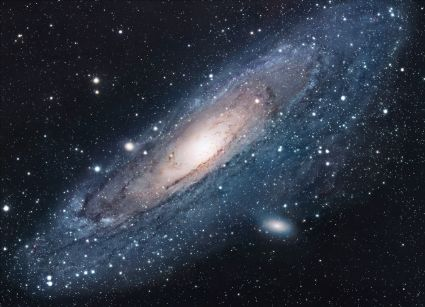
\includegraphics[scale=1.7]{universe.jpg}
\caption{The Universe}
\label{fig:univerise}
\end{figure}


\section{De Descartes a Popper em um piscar de olhos}


\section{O método científico}

\subsection{xxxxxx}

\subsection{yyyyyy}

\section{Conclusão}
``I always thought something was fundamentally wrong with the universe'' \citep{adams1995hitchhiker}

\bibliographystyle{plain}
\bibliography{references}
\end{document}
